%Este trabalho está licenciado sob a Licença Atribuição-CompartilhaIgual 4.0 Internacional Creative Commons. Para visualizar uma cópia desta licença, visite http://creativecommons.org/licenses/by-sa/4.0/deed.pt_BR ou mande uma carta para Creative Commons, PO Box 1866, Mountain View, CA 94042, USA.

\chapter{Equações e inequações}\label{cap_ineq}
\thispagestyle{fancy}

\begin{flushright}
  [Vídeo] | [Áudio] | \href{https://phkonzen.github.io/notas/contato.html}{[Contatar]}
\end{flushright}

\section{Equações}\label{cap_ineq_sec_eq}

Uma equação é uma declaração de que duas expressões são iguais. Escrevemos
\begin{equation}
  E_{\text{esq}} = E_{\text{dir}}
\end{equation}
para estabelecer que a expressão à esquerda $E_{\text{esq}}$ é igual a expressão à direita $E_{\text{dir}}$.

\begin{ex}
  Estudemos os seguintes casos:
  \begin{enumerate}[a)]
  \item $2^2 = 4$
  \item $2x - 1 = 0$
  \item $e^{x+y} = e^xe^y$
  \item $\displaystyle \frac{x^2-1}{x+1} = x - 1$
  \end{enumerate}

  \begin{ifispython}
    No \python, podemos declarar as equações com a função \lstinline{https://docs.sympy.org/latest/modules/core.html?highlight=equality#sympy.core.relational.Equality}{Eq}. Os casos são implementados como segue:
    \begin{lstlisting}
      >>> from sympy import *
      >>> Eq(2**2, 4)
      True
      >>> x = Symbol('x')
      >>> Eq(2*x - 1, 0)
      Eq(2*x - 1, 0)
      >>> y = Symbol('y')
      >>> Eq(exp(x+y), exp(x)*exp(y))
      Eq(exp(x + y), exp(x)*exp(y))
      >>> Eq((x**2-1)/(x+1), x-1)
      Eq((x**2 - 1)/(x + 1), x - 1)
    \end{lstlisting}
  \end{ifispython}
\end{ex}

\subsection{Solução de uma equação}

Equação é uma poderosa ferramenta matemática para impor uma condição sobre uma ou mais \emph{incógnitas} (ou \emph{variáveis}). Por exemplo, quando escrevemos
\begin{equation}
  2^x = 4
\end{equation}
estamos impondo que a incógnita $x$ seja aquela a satisfazer esta equação. No caso, $x=2$ satisfaz a equação, pois ao substituirmos $x$ por $2$ nela, obtemos
\begin{gather}
  2^2 = 4
  \Leftrightarrow 4 = 4.
\end{gather}
Usualmente, dizemos que $x=2$ é \emph{solução} da equação. O procedimento de encontrar a(s) solução(ões) de uma equação é chamado de \emph{resolução} da equação, i.e. o procedimento de resolver a equação.

\begin{obs}
  Uma equação pode ter uma única solução, várias soluções, infinitas soluções ou nenhuma solução.
\end{obs}

\begin{ex}
  Estudemos os seguintes casos:
  \begin{enumerate}[a)]
  \item $x - 1 = 0$ tem solução única $x=1$.
  \item $y^2 - 1 = 0$ têm soluções $y=-1$ ou $y=1$.
  \item $x^2 = -1$ não tem solução.
  \item $(u+1)^2 = u^2 + 2u + 1$, qualquer $u\in\mathbb{R}$ é solução.
  \end{enumerate}

  \ifispython
  No \python, podemos resolver estas equações com o comando \href{https://docs.sympy.org/latest/tutorial/solvers.html#solving-equations-algebraically}{solve ou solveset}. Estudemos as seguintes entradas e saídas:
  \begin{lstlisting}
    >>> from sympy import *
    >>> x = Symbol('x', real=True)
    >>> solve(x-1, domain=S.Reals)
    [1]
    >>> solveset(x-1, domain=S.Reals)
    FiniteSet(1)
    >>> y,u = symbols('y,u', real=True)
    >>> solve(y**2-1, domain=S.Reals)
    [-1, 1]
    >>> solve(Eq(x**2, -1), domain=S.Reals)
    []
    >>> solveset(Eq(x**2, -1), domain=S.Reals)
    EmptySet
    >>> solveset(Eq((u+1)**2, u**2 + 2*u + 1), domain=S.Reals)
    Reals
  \end{lstlisting}
  \fi
\end{ex}

Não existe um procedimento único para a resolução de equações em geral. Em síntese, a resolução, quando possível, é obtida da aplicação das seguintes propriedades. Sendo $E_1$, $E_2$ e $E_3$ expressões matemáticas, temos
\begin{itemize}
\item Simetria
  \begin{equation}
    \begin{gathered}
      E_1 = {\color{blue}E_2} \\
      \Leftrightarrow \\
      {\color{blue}E_2} = E_1
    \end{gathered}
\end{equation}
\item Cancelamento por adição
  \begin{equation}
    \begin{gathered}
      E_1 = E_2 \\
      \Leftrightarrow \\
      E_1 + {\color{blue}E_3} = E_2 + {\color{blue}E_3}
  \end{gathered}
\end{equation}
\item Cancelamento por multiplicação\footnote{Somente no caso de $E_3\in\mathbb{R}^*$}
  \begin{equation}
    \begin{gathered}
      E_1 = E_2 \\
      \Leftrightarrow \\
      E_1\cdot {\color{blue}E_3} = E_2 \cdot {\color{blue}E_3}
  \end{gathered}
  \end{equation}
\end{itemize}

As operações acima reescrevem a equação original $E_1 = E_2$ em \emph{equações equivalentes}, i.e. equações que têm as mesmas soluções.

\begin{ex}
  Estudemos os casos a seguir.
  \begin{enumerate}[a)]
  \item
    \begin{gather}
      -1 = x\\
      x = -1
    \end{gather}
  \item
    \begin{gather}
      x - 2 = 1\\
      x - 2 {\color{blue}+ 2} = 1 {\color{blue}+ 2}\\
      x = 3
    \end{gather}
  \item
    \begin{gather}
      2x = 4\\
      {\color{blue}\frac{1}{2}\cdot}2x = {\color{blue}\frac{1}{2}\cdot}4\\
      1\cdot x = 2\\
      x = 2
    \end{gather}
  \end{enumerate}
\end{ex}

\subsection{Equações lineares}

Equação algébricas lineares de uma incógnita são aquelas que podem ser escritas na seguinte forma
\begin{equation}
  ax + b = 0,
\end{equation}
onde, são conhecidos (dados) os \emph{coeficientes} $a\in\mathbb{R}^*$ e $b\in\mathbb{R}$. Sua resolução pode ser feita da seguinte forma
\begin{gather}
  ax + b = 0 \\
  ax + b {\color{blue}- b} = 0 {\color{blue}- b} \\
  ax = -b \\
  {\color{blue}\frac{1}{a}\cdot}ax = {\color{blue}\frac{1}{a}\cdot}(-b) \\
  1\cdot x = -\frac{b}{a} \\
  {\color{blue}x = -\frac{b}{a}}
\end{gather}

\begin{ex}
  Vamos resolver
  \begin{equation}
    2x -4 = 5 - x
  \end{equation}
  Esta é uma equação linear, pois
  \begin{gather}
    2x - 4 {\color{blue}- 5} = 5 - x {\color{blue}- 5} \\
    2x -9 = -x \\
    {\color{blue}x} + 2x - 9 = {\color{blue}x} - x \\
    3x - 9 = 0\\
  \end{gather}
  Logo, a solução é
  \begin{equation}
    x = \frac{9}{3} = 3.
  \end{equation}

  \ifispython
  No \python, podemos resolver esta equação com
  \begin{lstlisting}
    >>> from sympy import *
    >>> x = Symbol('x', real=True)
    >>> solve(Eq(2*x - 4, 5 - x), domain=S.Reals)
    [3]
  \end{lstlisting}
  \fi
\end{ex}

\subsection{Equação quadrática}

Uma equação algébrica quadrática de um incógnita é aquela que pode ser escrita na forma
\begin{equation}\label{eq:ineq_eqq}
  ax^2 + bx + c = 0,
\end{equation}
com $a\in\mathbb{R}^*$ e $b,c\in\mathbb{R}$.

Para resolver tal equação, vamos, primeiro, lembrar que
\begin{equation}\label{eq:ineq_qp}
  (a + b)^2 = a^2 + 2ab + b^2,
\end{equation}
para quaisquer $a,b\in\mathbb{R}$. A ideia é usar desta \emph{identidade}\footnote{Identidade é o nome dado a uma equação que é satisfeita para todos os possíveis valores de sua(s) incógnita(s).} para reduzirmos a equação em duas equações lineares.

Começamos reescrevendo \eqref{eq:ineq_eqq} da seguinte forma
\begin{gather}
  ax^2 + bx + c {\color{blue}- c} = 0 {\color{blue}- c}\\
  ax^2 + bx = -c\\
  \left(ax^2 + bx\right){\cdot \color{blue}\frac{1}{a}} = -c{\cdot \color{blue}\frac{1}{a}} \\
  x^2 + \frac{b}{a}x = -\frac{c}{a}
\end{gather}
Agora, vamos \emph{completar os quadrados} do lado direito para usarmos a identida \eqref{eq:ineq_qp}. Fazemos
\begin{gather}
  x^2 + \frac{b}{a}x {\color{blue}+ \left(\frac{b}{2a}\right)^2} = -\frac{c}{a}  {\color{blue}+ \left(\frac{b}{2a}\right)^2} \\
  \left(x + \frac{b}{2a}\right)^2 = -\frac{c}{a} + \frac{b^2}{4a^2} \\
  \left(x + \frac{b}{2a}\right)^2 = \frac{b^2 - 4ac}{4a^2}
\end{gather}
Agora, extraímos a raiz quadrada de ambos os lados da equação\footnote{$\sqrt{x^2}=|x|$.}
\begin{gather}
  \sqrt{\left(x + \frac{b}{2a}\right)^2} = \sqrt{\frac{b^2 - 4ac}{4a^2}} \\
  \left|x + \frac{b}{2a}\right| = \left|\frac{\sqrt{b^2 - 4ac}}{2a}\right|
\end{gather}
Daí, seguem as seguintes equações lineares
\begin{gather}
  x + \frac{b}{2a} = \frac{\sqrt{b^2 - 4ac}}{2a}\\
  {\color{blue}\text{ou}}\nonumber\\
  x + \frac{b}{2a} = -\frac{\sqrt{b^2 - 4ac}}{2a}\\
\end{gather}
Equivalentemente, escrevemos
\begin{equation}
  x + \frac{b}{2a} = \pm\frac{\sqrt{b^2 - 4ac}}{2a}
\end{equation}
Por fim, isolamos $x$ co
\begin{equation}
  x = -\frac{b}{2a} \pm\frac{\sqrt{b^2 - 4ac}}{2a}
\end{equation}
donde temos a chamada \emph{Fórumla de Bhaskara}\footnote{Bhaskara Akaria, 1114 - 1185, matemático indiano. Fonte: \href{https://pt.wikipedia.org/wiki/Bhaskara\_II}{Wikipédia}.}
\begin{equation}\label{eq:ineq_bhaskara}
  x = \frac{-b \pm \sqrt{b^2 - 4ac}}{2a}.
\end{equation}

\begin{ex}
  Vamos resolver
  \begin{equation}
    x^2 = x + 2.
  \end{equation}
  Esta é uma equação quadrática, pois
  \begin{gather}
    x^2 {\color{blue}- x - 2} = x + 2 {\color{blue}- x - 2} \\
    x^2 -x - 2 = 0.
  \end{gather}
  Logo, da Fórmula da Bhaskara \eqref{eq:ineq_bhaskara}, obtemos
  \begin{gather}
    x = \frac{-(-1) \pm \sqrt{(-1)^2 - 4\cdot 1 \cdot (-2)}}{2\cdot 1} \\
    x = \frac{1 \pm \sqrt{1 + 8}}{2} \\
    x = \frac{1 \pm \sqrt{9}}{2} \\
    x = \frac{1 \pm 3}{2}
  \end{gather}
  Donde,
  \begin{gather}
    x = \frac{1 - 3}{2} \\
    x = \frac{-2}{2} \\
    x = -1
  \end{gather}
  ou
  \begin{gather}
    x = \frac{1 + 3}{2} \\
    x = \frac{4}{2} \\
    x = 2
  \end{gather}
  Concluímos que a equação tem soluções $x=-1$ ou $x=2$.

  \ifispython
  No \python, podemos resolver esta equação com
  \begin{lstlisting}
    >>> from sympy import *
    >>> x = Symbol('x', real=True)
    >>> solve(Eq(x**2, x + 2), domain=S.Reals)
    [-1, 2]
  \end{lstlisting}
  \fi
\end{ex}

\subsection{Equações exponenciais}

Um equação exponencial é aquela em que a incógnita aparece como expoente em um ou mais termos. Tais equações não tem formato único, nem procedimento geral de resolução. Quando possível, a ideia é reescrever todos os termos da equação em uma base comum.

\begin{obs}
  Lembramos que\footnote{Quando bem definido.}:
  \begin{itemize}
  \item $\displaystyle b^x = b^y \Leftrightarrow x=y$
  \item $\displaystyle b^{x+y} = b^x\cdot b^y$
  \item $\displaystyle b^{xy} = \left(b^x\right)^y$
  \item $\displaystyle b^{-x} = \frac{1}{b^x}$
  \item $\displaystyle b^{\frac{x}{y}} = \sqrt[y]{b^x}$
  \end{itemize}
\end{obs}

\begin{ex}
  Vamos resolver
  \begin{equation}
    5^{x+3} = 25.
  \end{equation}
  Para resolver esta equação, vamos escrever $25$ como potência de $5$, i.e.
  \begin{equation}
    25 = 5^2.
  \end{equation}
  Logo, a equação é equivalente a
  \begin{equation}
    5^{x+3} = 5^2
  \end{equation}
  donde
  \begin{gather}
    x+3 = 2 \\
    x = -1.
  \end{gather}
  Ou seja, a solução é $x=-1$.

  \ifispython
  No \python:
  \begin{lstlisting}
    >>> from sympy import *
    >>> x = Symbol('x', real=True)
    >>> solve(Eq(5**(x+3), 25), domain=S.Reals)
    [-1]
  \end{lstlisting}
  \fi
\end{ex}

\begin{ex}
  Vamos resolver
  \begin{equation}
    5^{x+3} = 5^{-x} + 20.
  \end{equation}
  Notamos que esta equação é equivalente a
  \begin{equation}
    5^x\cdot 5^3 = \left(5^x\right)^{-1} + 20.
  \end{equation}
  Fazemos, então, a seguinte \emph{mudança de variável}
  \begin{equation}
    y = 5^x.
  \end{equation}
  Com isso, a equação se resume a
  \begin{equation}
    y\cdot 5^3 = y^{-1} + 20
  \end{equation}
  Resolvemos esta equação como segue
  \begin{gather}
    125y = \frac{1}{y} + 20 \\
    125y^2 = 1 + 20y \\
    125y^2 - 20y - 1 = 0
  \end{gather}
  Usando a fórmula de Bhaskara, obtemos
  \begin{gather}
    y = \frac{20 \pm \sqrt{20^2 - 4\cdot 125\cdot (-1)}}{2\cdot 125}\\
    y = \frac{20 \pm \sqrt{900}}{250} \\
    y = \frac{20 - \pm 30}{250}
  \end{gather}
  Ou seja, $y = -1/25$ ou $y = 1/5$. Observando que $y=5^x$ e, portanto positivo, temos
  \begin{equation}
    5^x = \frac{1}{5} = 5^{-1}.
  \end{equation}
  Concluímos que $x = -1$.

  \ifispython
  No \python:
  \begin{lstlisting}
    >>> from sympy import *
    >>> x = Symbol('x', real=True)
    >>> solveset(Eq(5**(x+3), 5**(-x) + 20), domain=S.Reals)
    [-1]
  \end{lstlisting}
  \fi  
\end{ex}

\subsection*{Exercícios}

\begin{exer}
  Calcule a solução das seguintes equações:
  \begin{enumerate}[a)]
  \item $x - 2 = 0$
  \item $3 - x = 1$
  \item $0 = -1 + x$
  \item $\sqrt{2}\cdot x = 0$
  \end{enumerate}
\end{exer}
\begin{resp}
  a) $2$; b) $2$; c) $1$; d) $0$
\end{resp}

\begin{exer}
  Calcule a solução das seguintes equações:
  \begin{enumerate}[a)]
  \item $2x - 3 = 2$
  \item $2x - 3 = 2 - x$
  \item $x - 3 = 2 + 2x$
  \end{enumerate}
\end{exer}
\begin{resp}
  a) $\frac{5}{2}$; b) $\frac{5}{3}$; c) $5$
\end{resp}

\begin{exer}
  Calcule a solução das seguintes equações:
  \begin{enumerate}[c)]
  \item $x^2 = 0$
  \item $x^2 + 4 = 0$
  \item $x^2 + 4x + 4 = 0$
  \item $x^2 - 16 = 0$
  \item $x^2 + x - 2 = 0$
  \item $2x - 6 + x^2 = -x^2 - 2$
  \end{enumerate}
\end{exer}
\begin{resp}
  a) $0$; b) $\nexists$; c) $-2$; d) $\{-4,4\}$; e) $\{-2,1\}$; f) $\{-2,1\}$ 
\end{resp}

\begin{exer}
  Calcule a solução das seguintes equações:
  \begin{enumerate}
  \item $3^x = 27$
  \item $2^x = 2\cdot 2^x - 1$
  \item $4^x = 2 - 2^x$
  \end{enumerate}
\end{exer}
\begin{resp}
 a) $3$; b) $0$; c) $0$
\end{resp}

\begin{exer}
  Calcule a solução da seguinte equação
  \begin{equation}
    x^4 - 2x^2 + 1 = 0
  \end{equation}
\end{exer}
\begin{resp}
  $\{-1,1\}$
\end{resp}

\section{Inequações}\label{cap_ineq_sec_ineq}

Uma inequação é uma sentença matemática que expressa uma relação de desigualdade entre duas expressões matemáticas. São exemplos de inequações
\begin{gather}
  E_{\text{esq}} \neq E_{\text{dir}}\\
  E_{\text{esq}} < E_{\text{dir}}\\
  E_{\text{esq}} \leq E_{\text{dir}}\\
  E_{\text{esq}} > E_{\text{dir}}\\
  E_{\text{esq}} \geq E_{\text{dir}}
\end{gather}
Assim como equações, inequações são usadas para descrever propriedades ou restrições sobre uma ou mais incógnitas. Neste caso, a \emph{solução} é o conjunto de valores que a incógnita pode assumir de forma a satisfazer a inequação.

\begin{ex}
  São exemplos de inequações envolvendo incógnitas:
  \begin{enumerate}[a)]
  \item Inequação de primeiro grau
    \begin{equation}
      2x + 3 > 5
    \end{equation}
  \item Inequação de segundo grau
    \begin{equation}
      x^2 \leq x - 3
    \end{equation}
  \item Inequação racional
    \begin{equation}
      \frac{2x + 3}{x^2} \geq \frac{5}{x-3}
    \end{equation}
  \end{enumerate}
\end{ex}

Não existe um procedimento geral para calcular a solução de uma inequação, mas o chamado estudo de sinal pode ser uma estratégia adequada em várias situações. Na sequência, vamos aplicá-la na resolução de algumas inequações.

\subsection{Inequações de primeiro grau}

Inequações de primeiro grau são aquelas em que a incógnita aparece apenas na potência 1. Ou seja, qualquer inequação que possa ser escrita na seguinte forma
\begin{equation}\label{eq:ineq_g1}
  ax + b \gtreqless 0,
\end{equation}
onde $a,b\in\mathbb{R}$, $a\neq 0$, são coeficientes/parâmetros dados e $x$ é a incógnita.

Para resolvê-la, podemos usar o \emph{estudo de sinal} da expressão\footnote{Lembremos a tricotomia dos números reais. Consulte a Subseção \ref{ssec:numreal_retareal}.} $ax + b$. Para que seja nula, temos
\begin{gather}
  ax + b = 0
  \Leftrightarrow
  x = -\frac{b}{a}
\end{gather}
Com isso, observamos que no caso de ${\color{blue}a>0}$, temos que
\begin{equation}
  x{\color{blue}>}-\frac{b}{a} \Rightarrow ax + b {\color{blue}>} 0
\end{equation}
e
\begin{equation}
  x {\color{red}<} -\frac{b}{a} \Rightarrow ax + b {\color{red}<} 0.
\end{equation}
Consultemos a Figura \ref{fig:ineq_g1ap}.

\begin{figure}[H]
  \centering
  \includegraphics{./cap_ineq/dados/fig_ineq_g1ap/fig}
  \caption{Representação geométrica do estudo do sinal de $ax + b$, com $a>0$.}
  \label{fig:ineq_g1ap}
\end{figure}

Agora, no caso de ${\color{red}a<0}$, temos
\begin{equation}
  x{\color{blue}>}-\frac{b}{a} \Rightarrow ax + b {\color{red}<} 0
\end{equation}
e
\begin{equation}
  x {\color{red}<} -\frac{b}{a} \Rightarrow ax + b {\color{blue}>} 0.
\end{equation}
Consultemos a Figura \ref{fig:ineq_g1an}.

\begin{figure}[H]
  \centering
  \includegraphics{./cap_ineq/dados/fig_ineq_g1an/fig}
  \caption{Representação geométrica do estudo do sinal de $ax + b$, com $a<0$.}
  \label{fig:ineq_g1an}
\end{figure}

\begin{ex}
  Vamos resolver
  \begin{equation}
    4 + x \geq -x
  \end{equation}
  Primeiramente, vamos reescrever a inequação no formato da \eqref{eq:ineq_g1}. Para tanto, calculamos
  \begin{gather}
    4 + x \pmb{+ x} \geq - x \pmb{ + x}\\
    4 + 2x \geq 0\\
    2x + 4 \geq 0
  \end{gather}

\begin{figure}[H]
  \centering
  \includegraphics{./cap_ineq/dados/fig_ex_ineq_g1ap/fig}
  \caption{Estudo do sinal de $2x + 4$.}
  \label{fig:ex_ineq_g1ap}
\end{figure}  
  
  Agora, fazemos o estudo de sinal de $2x + 3$. Temos
  \begin{equation}
    2x + 4 = 0 \Rightarrow x = -2.
  \end{equation}
  Daí, segue que
  \begin{equation}
    x > -2 \Rightarrow 2x + 4 > 0
  \end{equation}
  e
  \begin{equation}
    x < -2 \Rightarrow 2x + 4 < 0
  \end{equation}
  Consulte a Figura \ref{fig:ex_ineq_g1ap}. Logo, concluímos que a solução é $x\in [-2, \infty)$.

  \ifispython
  Com o {\sympy}, podemos computar a solução deste problema com os seguintes comandos
  \begin{lstlisting}
    >>> from sympy import *
    >>> x = symbols('x')
    >>> solve_univariate_inequality(4 + x >= -x, x)
    (-2 <= x) & (x < oo)
  \end{lstlisting}
  \fi
\end{ex}

Em alguns casos, é possível calcular a solução apenas a partir de manipulações algébricas.

\begin{ex}
  Vamos resolver
  \begin{equation}
    - 2x < 4
  \end{equation}
  Começamos multiplicando ambos os lados da inequação por $-1$ para obtermos\footnote{Notemos que a desigualdade se inverte ao multiplicarmos a inequação por um número negativo.}
  \begin{equation}
    2x > -4
  \end{equation}
  Agora, multiplicamos por $\frac{1}{2}$, como segue
  \begin{gather}
    \frac{1}{2}\cdot 2x > \frac{1}{2}\cdot (-4)\\
    x > -2
  \end{gather}
  Donde, temos a solução $x\in (-2, \infty)$.

  \begin{ifispython}
    Verifique usando o {\sympy}!
  \end{ifispython}
\end{ex}

\subsection{Produtos ou quocientes}

Inequações envolvendo produtos ou quocientes de expressões de primeiro grau podemos ser resolvidas fazendo-se o \emph{estudo de sinal}.

\begin{ex}
  Vamos resolver
  \begin{equation}
    (x - 1)(2 - x) < 0.
  \end{equation}
  
  \begin{figure}[H]
    \centering
    \includegraphics{./cap_ineq/dados/fig_ex_ineq_pg1/fig}
    \caption{Estudo do sinal de $(x-1)(2-x)$.}
    \label{fig:ex_ineq_pg1}
  \end{figure}  

  Para tanto, fazemos os estudos de sinais do primeiro fator $(x-1)$ e do segundo fator $(x+1)$. Em seguida, fazemos o estudo de sinal do produto $(x-1)(x+1)$. Neste caso, obtemos a Figura \ref{fig:ex_ineq_pg1}. Com isso, temos que a solução é $x\in (-\infty, 1)\cup (2, \infty)$.

  \begin{ifispython}
    Verifique usando o {\sympy}!
  \end{ifispython}
\end{ex}

No caso de quocientes, devemos nos atentar para o fato de que o denominador não seja nulo.

\begin{ex}
  Vamos resolver
  \begin{equation}
    \frac{x - 1}{2 - x} \geq 0.
  \end{equation}
  
  \begin{figure}[H]
    \centering
    \includegraphics{./cap_ineq/dados/fig_ex_ineq_qg1/fig}
    \caption{Estudo do sinal de $(x-1)/(2-x)$.}
    \label{fig:ex_ineq_qg1}
  \end{figure}  

  Para tanto, fazemos os estudos de sinais do primeiro fator $(x-1)$ e do segundo fator $(x+1)$. Em seguida, fazemos o estudo de sinal do quociente $(x-1)(x+1)$. Neste caso, obtemos a Figura \ref{fig:ex_ineq_qg1}. Com isso, temos que a solução é $x\in [1, 2)$.

  \begin{ifispython}
    Verifique usando o {\sympy}!
  \end{ifispython}
\end{ex}

\subsection*{Exercícios}

\begin{exer}
  Resolva as seguintes inequações
  \begin{enumerate}[a)]
  \item $x - 1 < 0$
  \item $2 - x \geq 0$
  \item $2 - 2x > 5$
  \item $3x + 2 \leq 3 - x$
  \end{enumerate}
\end{exer}
\begin{resp}
  a) $(-\infty, 1)$; b) $(-\infty, 2]$; c) $(-3/2, \infty)$; d) $(-\infty, 1/4]$
\end{resp}

\begin{exer}
  Resolva as seguintes inequações
  \begin{enumerate}
  \item $(x-2)(x+1) > 0$
  \item $(x-2)(1-x) \geq 0$
  \item $(x-2)(1-x) < 0$
  \item $(5x-2)(1-3x) \leq 0$
  \end{enumerate}
\end{exer}
\begin{resp}
  a) $(-\infty,-1)\cup (2,\infty)$; b) $[1,2]$; c) $(-\infty,1)\cup (2,\infty)$; d) $(-\infty,1/3]\cup [2/5,\infty)$
\end{resp}

\begin{exer}
  Resolva as seguintes inequações
  \begin{enumerate}
  \item $(x-2)/(x+1) > 0$
  \item $(x-2)/(1-x) \geq 0$
  \item $(x-2)/(1-x) < 0$
  \item $(5x-2)/(1-3x) \leq 0$
  \end{enumerate}
\end{exer}
\begin{resp}
  a) $(-\infty,-1)\cup (2,\infty)$; b) $(1,2]$; c) $(-\infty,1)\cup (2,\infty)$; d) $(-\infty,1/3)\cup [2/5,\infty)$
\end{resp}

\begin{exer}
  Resolva a seguinte inequação
  \begin{equation}
    x^2 - 4 < 0
  \end{equation}
\end{exer}
\begin{resp}
  $(-2,2)$
\end{resp}

\begin{exer}
  Resolve a seguinte inequação
  \begin{equation}
    \frac{x^2 + x - 2}{x+2} \geq 0
  \end{equation}
\end{exer}
\begin{resp}
  $(-\infty, -2)\cup (-2, 1]$
\end{resp}